% This file was created with tikzplotlib v0.10.1.
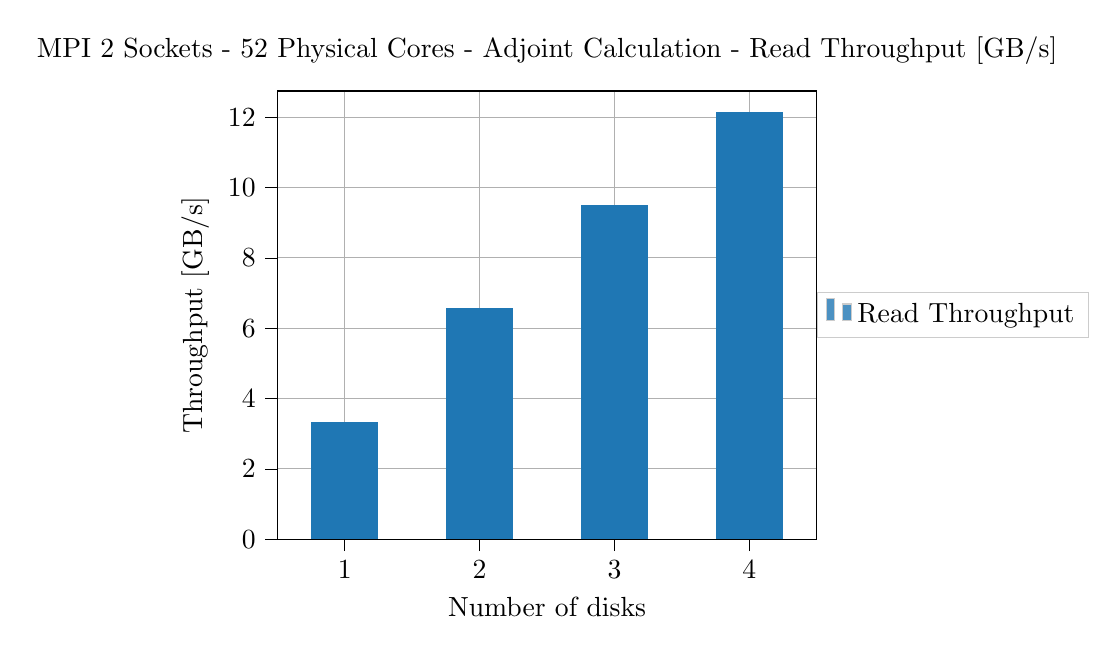
\begin{tikzpicture}

\definecolor{darkgray176}{RGB}{176,176,176}
\definecolor{lightgray204}{RGB}{204,204,204}
\definecolor{steelblue31119180}{RGB}{31,119,180}

\begin{axis}[
legend cell align={left},
legend style={
  fill opacity=0.8,
  draw opacity=1,
  text opacity=1,
  at={(1,0.5)},
  anchor=west,
  draw=lightgray204
},
tick align=outside,
tick pos=left,
title={MPI 2 Sockets - 52 Physical Cores - Adjoint Calculation - Read Throughput [GB/s]},
x grid style={darkgray176},
xlabel={Number of disks},
xmajorgrids,
xmin=-0.5, xmax=3.5,
xtick style={color=black},
xtick={0,1,2,3},
xticklabels={1,2,3,4},
y grid style={darkgray176},
ylabel={Throughput [GB/s]},
ymajorgrids,
ymin=0, ymax=12.7478328049088,
ytick style={color=black}
]
\draw[draw=none,fill=steelblue31119180] (axis cs:-0.25,0) rectangle (axis cs:0.25,3.32780545872029);
\addlegendimage{ybar,ybar legend,draw=none,fill=steelblue31119180}
\addlegendentry{Read Throughput}

\draw[draw=none,fill=steelblue31119180] (axis cs:0.75,0) rectangle (axis cs:1.25,6.58577997800289);
\draw[draw=none,fill=steelblue31119180] (axis cs:1.75,0) rectangle (axis cs:2.25,9.50387879874696);
\draw[draw=none,fill=steelblue31119180] (axis cs:2.75,0) rectangle (axis cs:3.25,12.1407931475322);
\end{axis}

\end{tikzpicture}
